%%%%%%%%%%%%%%%%%%%%%%%%%%%%%%%%%%%%%%%%%%%%%%%%%%%
%
%  New template code for TAMU Theses and Dissertations starting Fall 2012.  
%  For more info about this template or the 
%  TAMU LaTeX User's Group, see http://www.howdy.me/.
%
%  Author: Wendy Lynn Turner 
%	 Version 1.0 
%  Last updated 8/5/2012
%
%%%%%%%%%%%%%%%%%%%%%%%%%%%%%%%%%%%%%%%%%%%%%%%%%%%

%%%%%%%%%%%%%%%%%%%%%%%%%%%%%%%%%%%%%%%%%%%%%%%%%%%%%%%%%%%%%%%%%%%%%%
%%                           APPENDIX - DSA
%%%%%%%%%%%%%%%%%%%%%%%%%%%%%%%%%%%%%%%%%%%%%%%%%%%%%%%%%%%%%%%%%%%%%

\chapter{\uppercase {Extended MIP DSA Analysis}}
\label{sec::appendix_DSA}

In this appendix section, we will perform some additional analysis of the MIP diffusion form. We will assess the limits and nominal operational ranges of MIP in a lower dimensional space. Section \ref{sec::appendix_DSA_1D} will analyze the 1D MIP form while Section \ref{sec::appendix_DSA_2D} will analyze the 2D MIP form. For both 1D and 2D, Fourier Analysis along with some simple numerical studies are presented.

%%%%%%%%%%%%%%%%%%%%%%%%%%%%%%%%%%%%%%%%%%%%%%%%%%%
%%%%%%%%%%%%%%%%%%%%%%%%%%%%%%%%%%%%%%%%%%%%%%%%%%%
%%%   Section - 1D
%%%%%%%%%%%%%%%%%%%%%%%%%%%%%%%%%%%%%%%%%%%%%%%%%%%
%%%%%%%%%%%%%%%%%%%%%%%%%%%%%%%%%%%%%%%%%%%%%%%%%%%
\section{MIP Analysis in 1D}
\label{sec::appendix_DSA_1D}

\begin{equation}
\label{eq:1D_transport_eq}
\mu \frac{\partial \psi}{\partial x} + \sigma_t (x) \psi(x,\mu) = \frac{\sigma_s (x)}{2} \int_{-1}^{1} \psi(x,\mu') \, d\mu' + \frac{Q(x)}{2}
\end{equation}

\begin{equation}
\label{eq:1D_transport_discangle}
\mu_m \frac{\partial \psi_m}{\partial x} + \sigma_t (x) \psi_m (x)= \frac{\sigma_s (x)}{2} \sum_{m'=1}^{M} \psi_m (x) + \frac{Q(x)}{2}
\end{equation}

The linear, cell-wise elementary matrices for the mass, stiffness, and gradient matrices for cell $j$ are

\begin{equation}
\label{MIP_1D_matrices}
\begin{aligned}
	M_j =& \frac{1}{6h_j}
	\left[ \begin{array}{cc}
	2 & 1 \\
	1 & 2 
	\end{array} \right] ,\\
	K_j =& \frac{1}{h_j}
	\left[ \begin{array}{cc}
	1 & -1 \\
	-1 & 1 
	\end{array} \right] ,\\
	G_j =& \frac{1}{2}
	\left[ \begin{array}{cc}
	-1 & -1 \\
	 1 & 1 
	\end{array} \right] ,
\end{aligned}
\end{equation}

\noindent respectively.


\begin{equation}
\label{eq:1D_transport_discrete}
\mu_m \frac{\partial \psi}{\partial x} + \sigma_{t,j} \psi(x,\mu) = \frac{\sigma_s (x)}{2} \int_{-1}^{1} \psi(x,\mu') \, d\mu' + \frac{Q(x)}{2}
\end{equation}


%%%%%%%%%%%%%%%%%%%%%%%%%%%%%%%%%%%%%%%%%%%%%%%%%%%
%%%%%%%%%%%%%%%%%%%%%%%%%%%%%%%%%%%%%%%%%%%%%%%%%%%
%%%   SubSection - Fourier Results
\subsection{Fourier Analysis in 1D}
\label{sec::appendix_DSA_1D_Fourier}

\begin{equation}
\label{eq::1D_phase_matrix}
P = \left[ \begin{array}{cc}
	1 & 0 \\
	0 & e^{i \lambda h}
	\end{array} \right]
\end{equation}

\noindent where $i=\sqrt{-1}$.

%%%%%%%%%%%%%%%%%%%%%%%%%%%%%%%%%%%%%%%%%%%%%%%%%%%%%%
% Begin:1D Gauss Quadrature Plot

\begin{figure}
\label{fig::1D_gauss_quadrature}
\centering
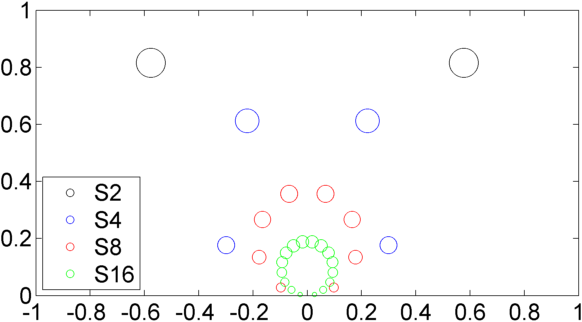
\includegraphics[width=\textwidth]{figures/appendices/1D_Gauss_Quad.png}
\caption{Visual representation of Gauss-Legendre quadrature sets.}
\end{figure}

% End: 1D Gauss Quadrature Plot
%%%%%%%%%%%%%%%%%%%%%%%%%%%%%%%%%%%%%%%%%%%%%%%%%%%%%%


%%%%%%%%%%%%%%%%%%%%%%%%%%%%%%%%%%%%%%%%%%%%%%%%%%%%%%
% Begin: IP and MIP 1D Fourier Plots

\begin{figure}
\label{fig::1D_IP_c=2}
\centering
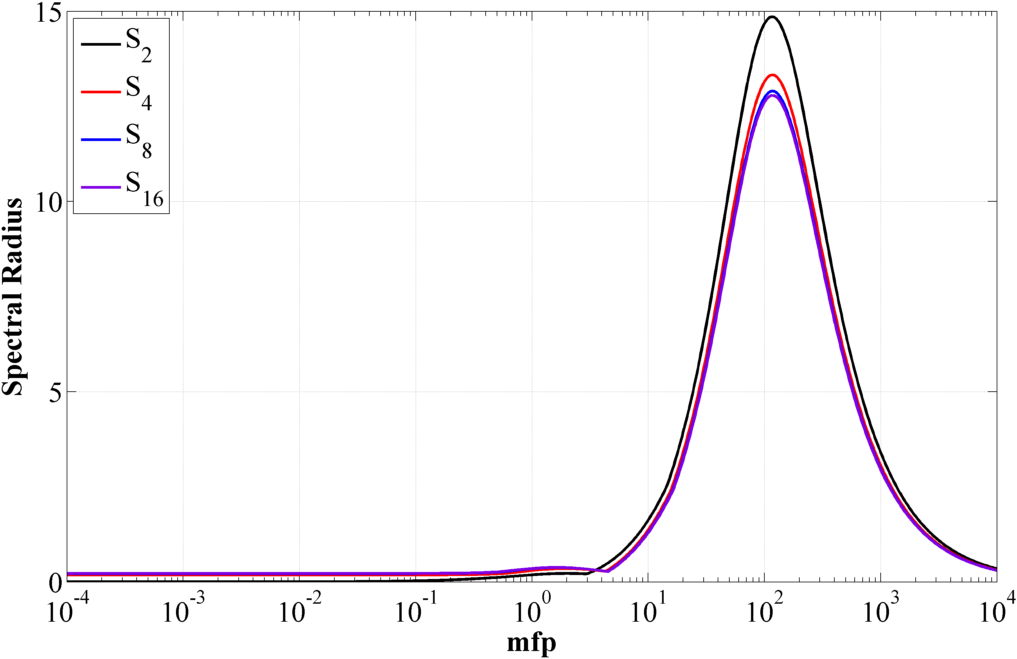
\includegraphics[width=0.98\textwidth]{figures/appendices/DSA_1D_SI_IP_C=2.png}
\caption{Spectral radius for the 1D IP form using $C=2$.}
\end{figure}

\begin{figure}
\label{fig::1D_IP_c=4}
\centering
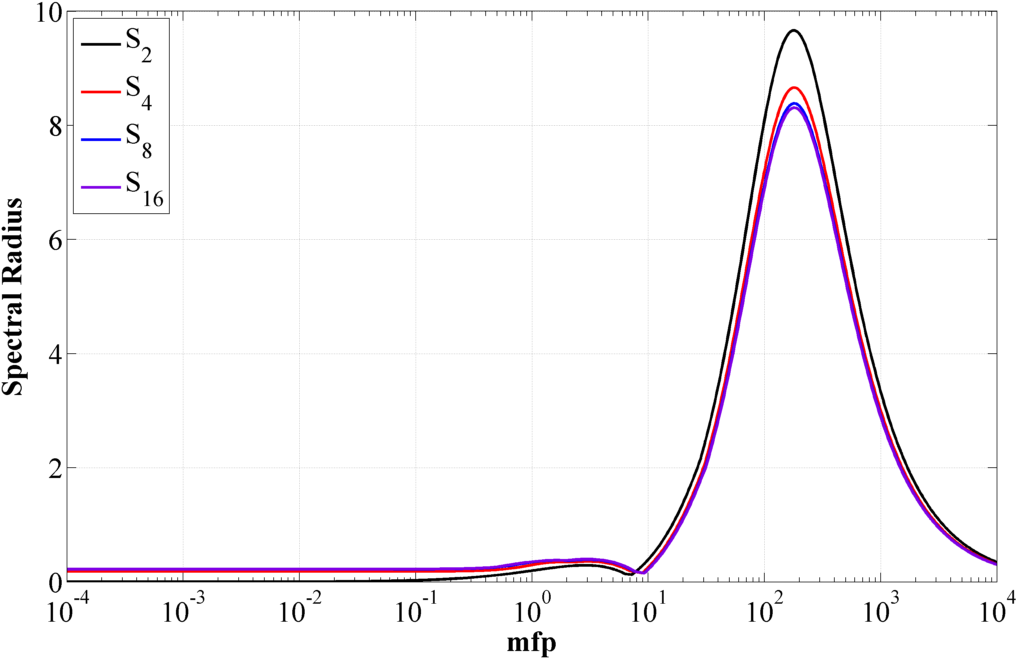
\includegraphics[width=0.98\textwidth]{figures/appendices/DSA_1D_SI_IP_C=4.png}
\caption{Spectral radius for the 1D IP form using $C=4$.}
\end{figure}

\begin{figure}
\label{fig::1D_IP_c=64}
\centering
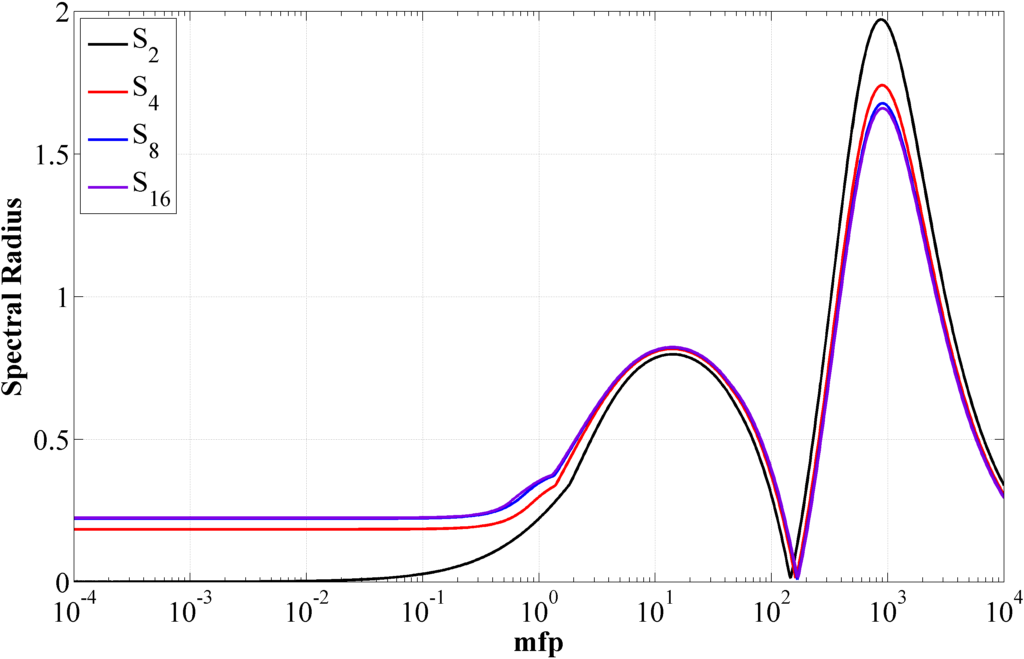
\includegraphics[width=0.98\textwidth]{figures/appendices/DSA_1D_SI_IP_C=64.png}
\caption{Spectral radius for the 1D IP form using $C=64$.}
\end{figure}

\begin{figure}
\label{fig::1D_IP_c=256}
\centering
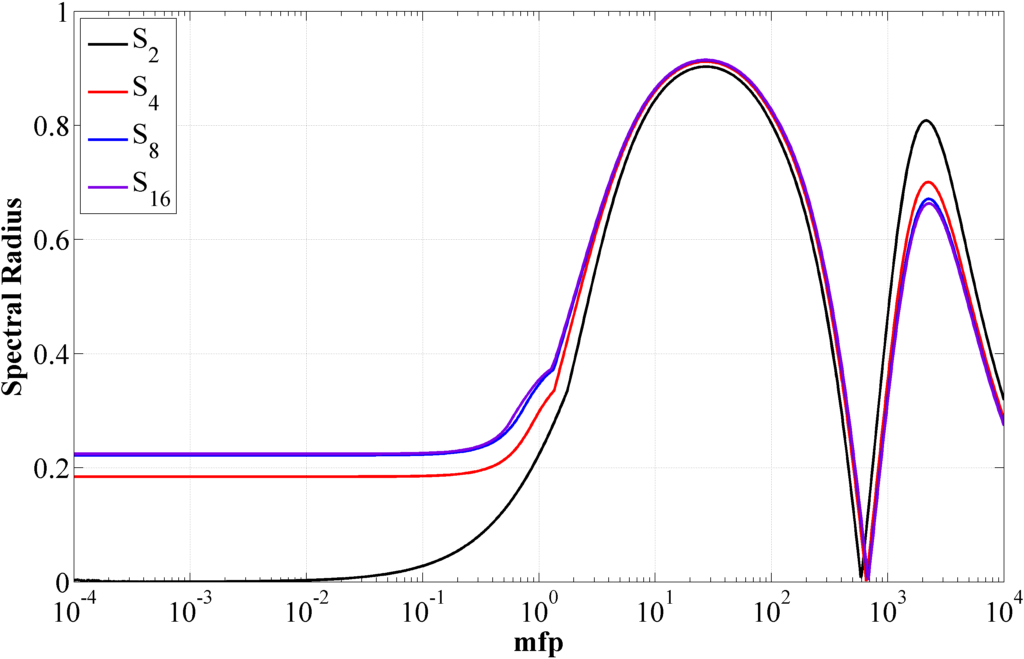
\includegraphics[width=0.98\textwidth]{figures/appendices/DSA_1D_SI_IP_C=256.png}
\caption{Spectral radius for the 1D IP form using $C=256$.}
\end{figure}

\begin{figure}
\label{fig::1D_MIP_c=1}
\centering
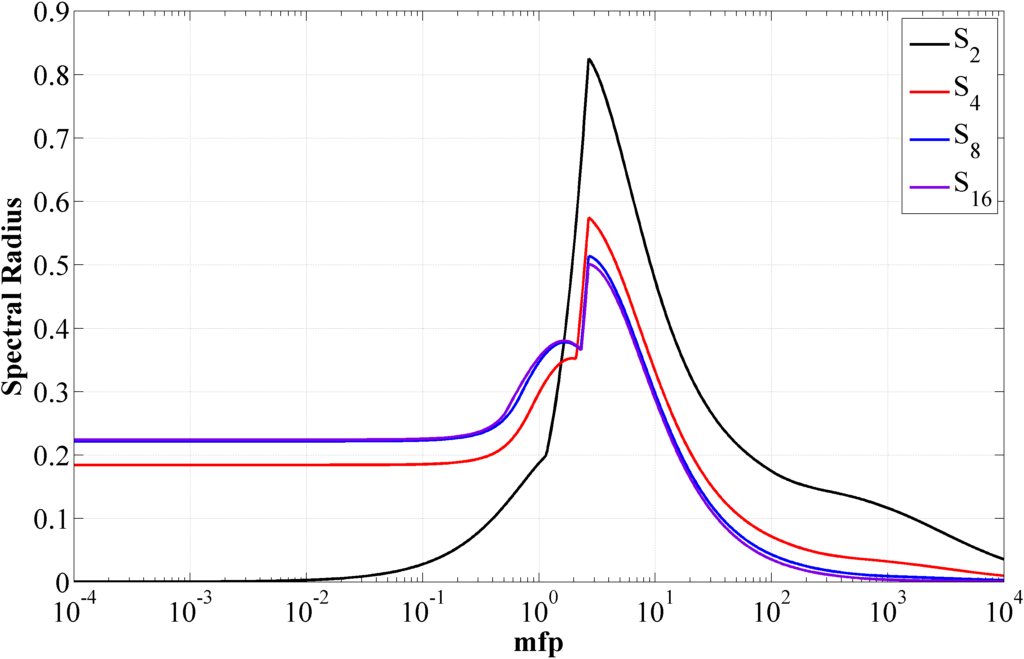
\includegraphics[width=\textwidth]{figures/appendices/DSA_1D_SI_MIP_C=1.png}
\caption{Spectral radius for the 1D MIP form using $C=1$.}
\end{figure}

\begin{figure}
\label{fig::1D_MIP_c=2}
\centering
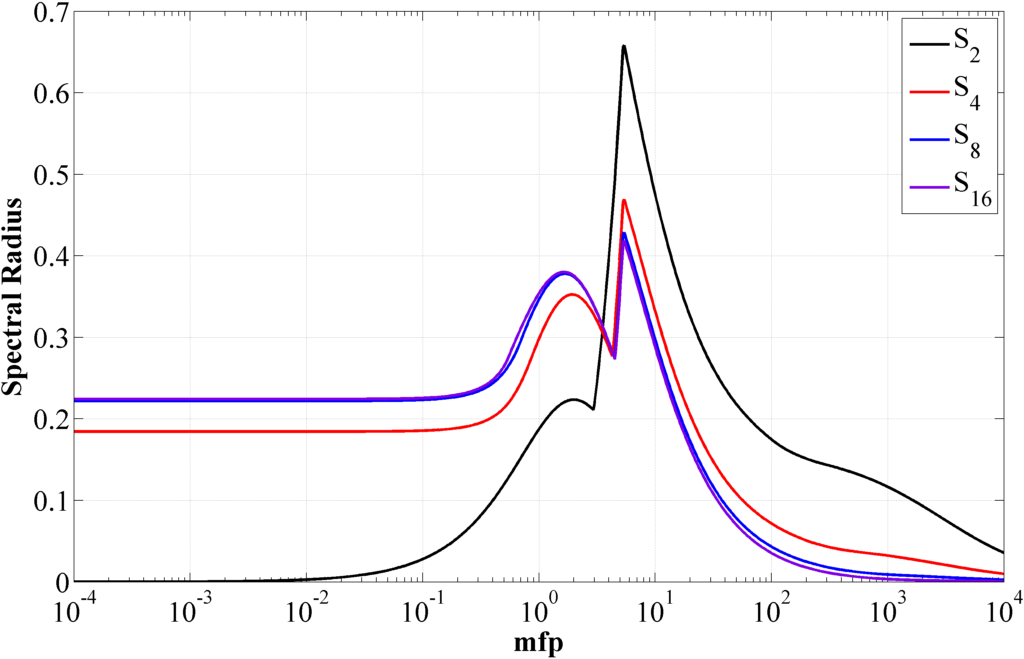
\includegraphics[width=\textwidth]{figures/appendices/DSA_1D_SI_MIP_C=2.png}
\caption{Spectral radius for the 1D MIP form using $C=2$.}
\end{figure}

\begin{figure}
\label{fig::1D_MIP_c=4}
\centering
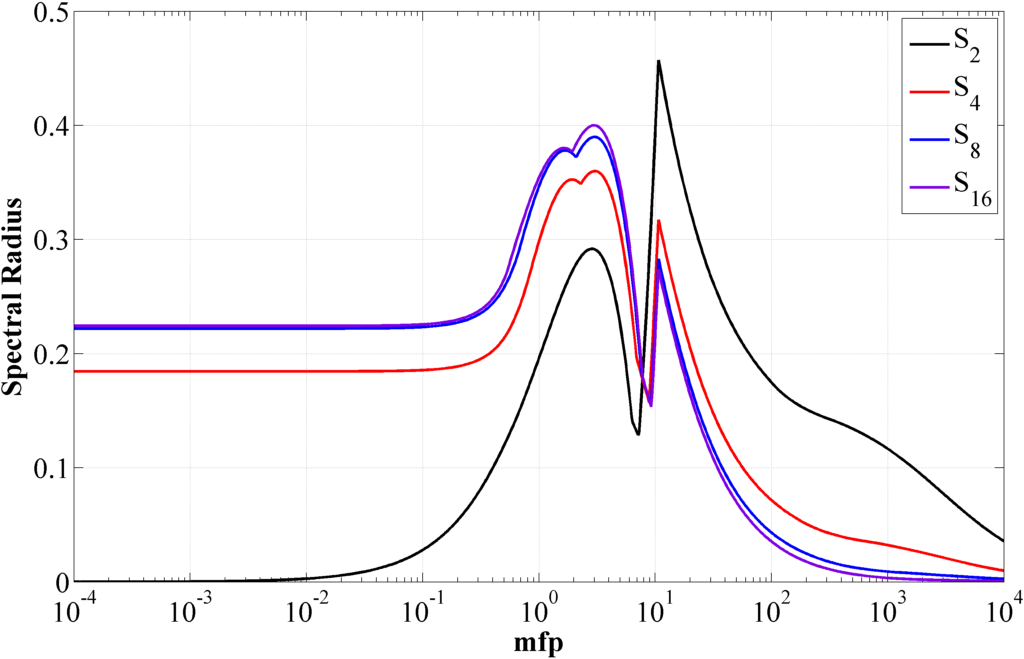
\includegraphics[width=\textwidth]{figures/appendices/DSA_1D_SI_MIP_C=4.png}
\caption{Spectral radius for the 1D MIP form using $C=4$.}
\end{figure}

\begin{figure}
\label{fig::1D_MIP_c=8}
\centering
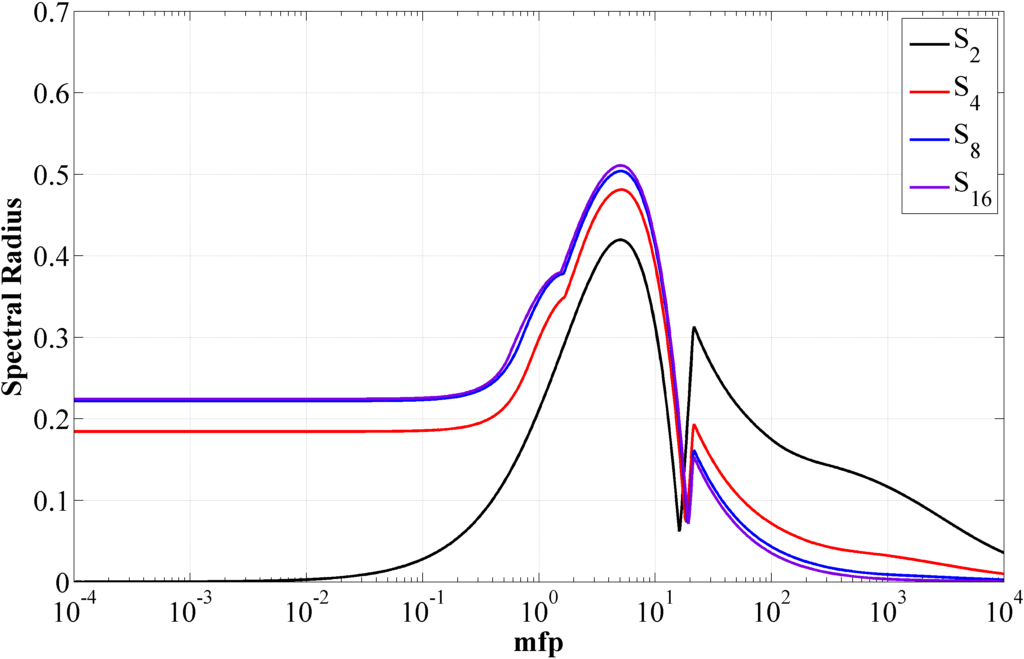
\includegraphics[width=\textwidth]{figures/appendices/DSA_1D_SI_MIP_C=8.png}
\caption{Spectral radius for the 1D MIP form using $C=8$.}
\end{figure}

\begin{figure}
\label{fig::1D_MIP_c=64}
\centering
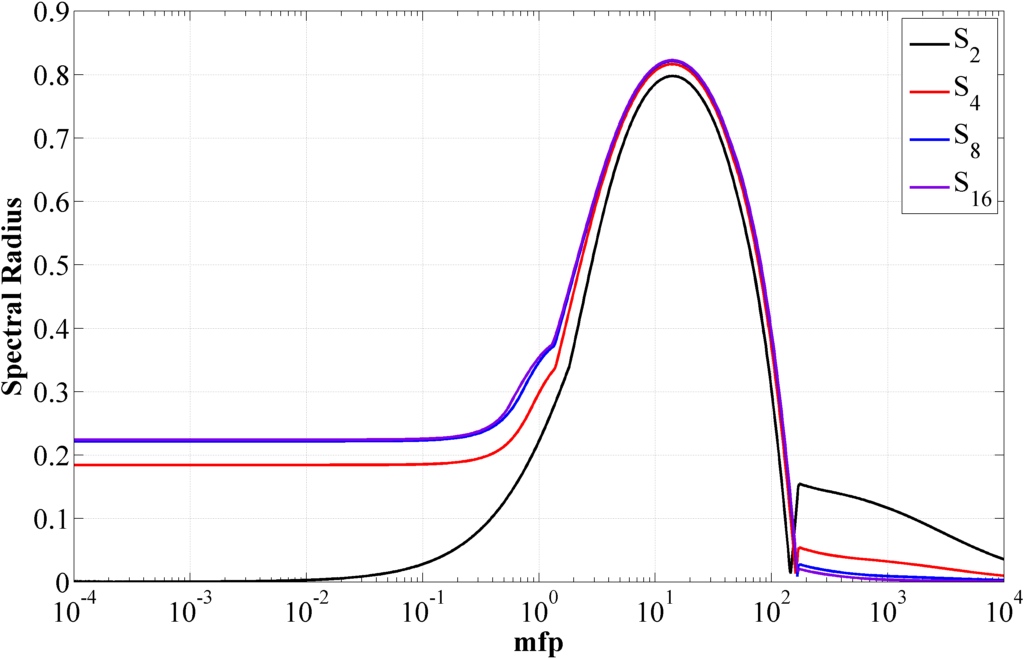
\includegraphics[width=\textwidth]{figures/appendices/DSA_1D_SI_MIP_C=64.png}
\caption{Spectral radius for the 1D MIP form using $C=64$.}
\end{figure}

\begin{figure}
\label{fig::1D_MIP_c=256}
\centering
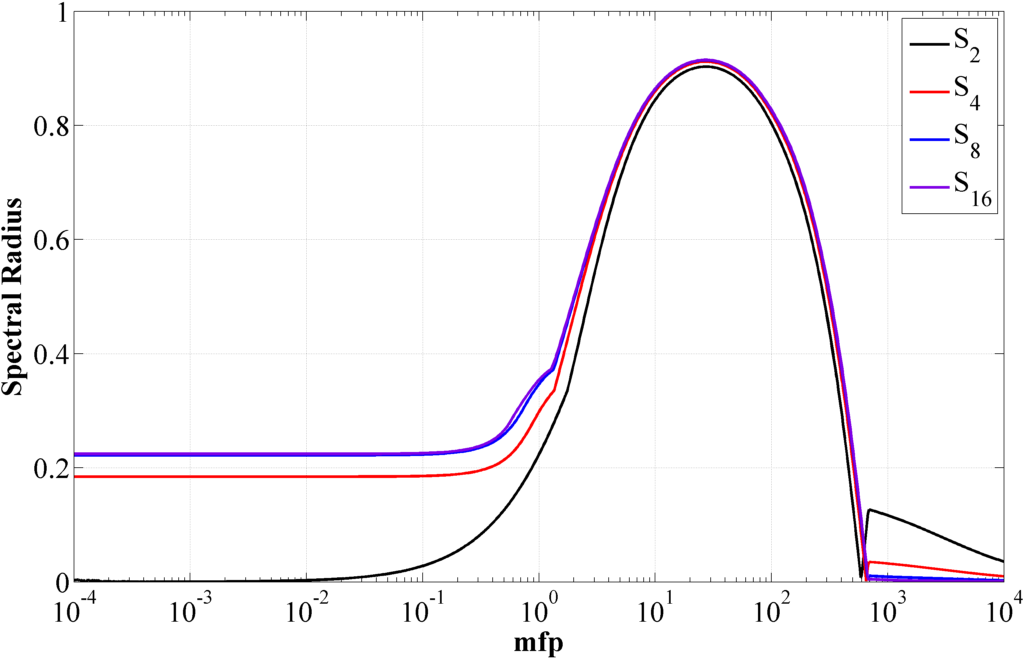
\includegraphics[width=\textwidth]{figures/appendices/DSA_1D_SI_MIP_C=256.png}
\caption{Spectral radius for the 1D MIP form using $C=256$.}
\end{figure}
% End: IP and MIP 1D Fourier Plots
%%%%%%%%%%%%%%%%%%%%%%%%%%%%%%%%%%%%%%%%%%%%%%%%%%%%%%


%%%%%%%%%%%%%%%%%%%%%%%%%%%%%%%%%%%%%%%%%%%%%%%%%%%
%%%%%%%%%%%%%%%%%%%%%%%%%%%%%%%%%%%%%%%%%%%%%%%%%%%
%%%   Section - 2D
%%%%%%%%%%%%%%%%%%%%%%%%%%%%%%%%%%%%%%%%%%%%%%%%%%%
%%%%%%%%%%%%%%%%%%%%%%%%%%%%%%%%%%%%%%%%%%%%%%%%%%%
\section{MIP Analysis in 2D}
\label{sec::appendix_DSA_2D}

%%%%%%%%%%%%%%%%%%%%%%%%%%%%%%%%%%%%%%%%%%%%%%%%%%%
%%%%%%%%%%%%%%%%%%%%%%%%%%%%%%%%%%%%%%%%%%%%%%%%%%%
%%%   SubSection - Fourier Results
\subsection{Fourier Analysis in 2D}
\label{sec::appendix_DSA_2D_Fourier}


%%%%%%%%%%%%%%%%%%%%%%%%%%%%%%%%%%%%%%%%%%%%%%%%%%%%%%
% Begin: IP and MIP 2D Fourier Plots


% End: IP and MIP 2D Fourier Plots
%%%%%%%%%%%%%%%%%%%%%%%%%%%%%%%%%%%%%%%%%%%%%%%%%%%%%%

%%%%%%%%%%%%%%%%%%%%%%%%%%%%%%%%%%%%%%%%%%%%%%%%%%%
%%%%%%%%%%%%%%%%%%%%%%%%%%%%%%%%%%%%%%%%%%%%%%%%%%%
%%%   SubSection - NSR Results
\subsection{Simple 2D Numerical Spectral Radius Analysis}
\label{sec::appendix_DSA_2D_NSR}



%%%%%%%%%%%%%%%%%%%%%%%%%%%%%%%%%%%%%%%%%%%%%%%%%%%%%%
% Begin: IP and MIP 2D NSR Plots

\begin{figure}
\label{fig::2D_NSR_MIP_quads}
\centering
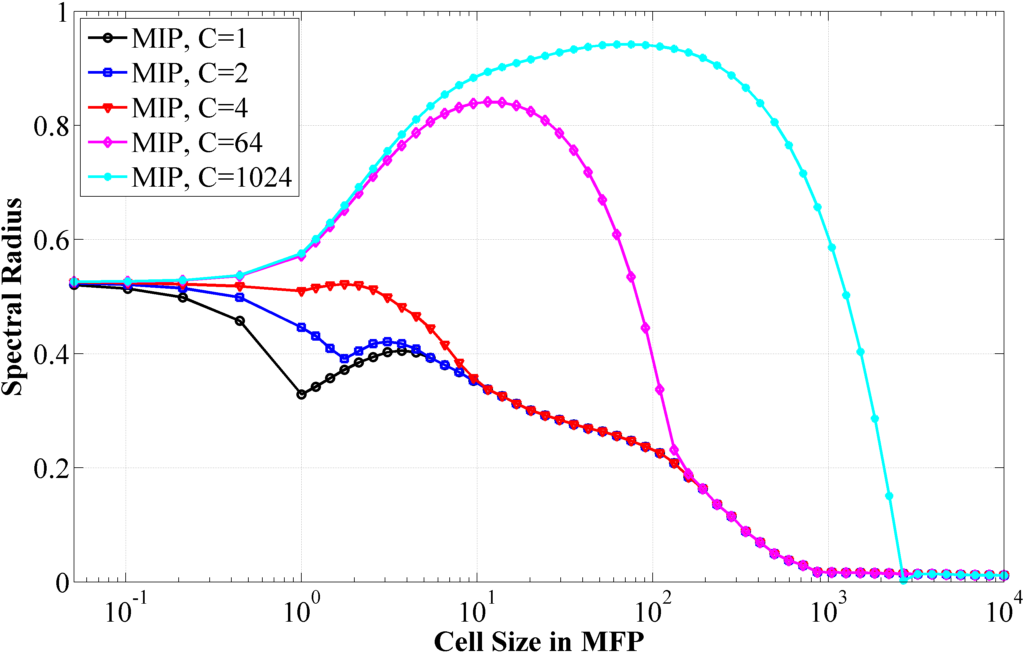
\includegraphics[width=0.9\textwidth]{figures/appendices/MIP_V_quad_LS8_C=1,2,4,64,1024.png}
\caption{Numerical spectral radius for the 2D MIP form using LS8 quadrature on quadrilaterals.}
\end{figure}

\begin{figure}
\label{fig::2D_NSR_MIP_triangles}
\centering
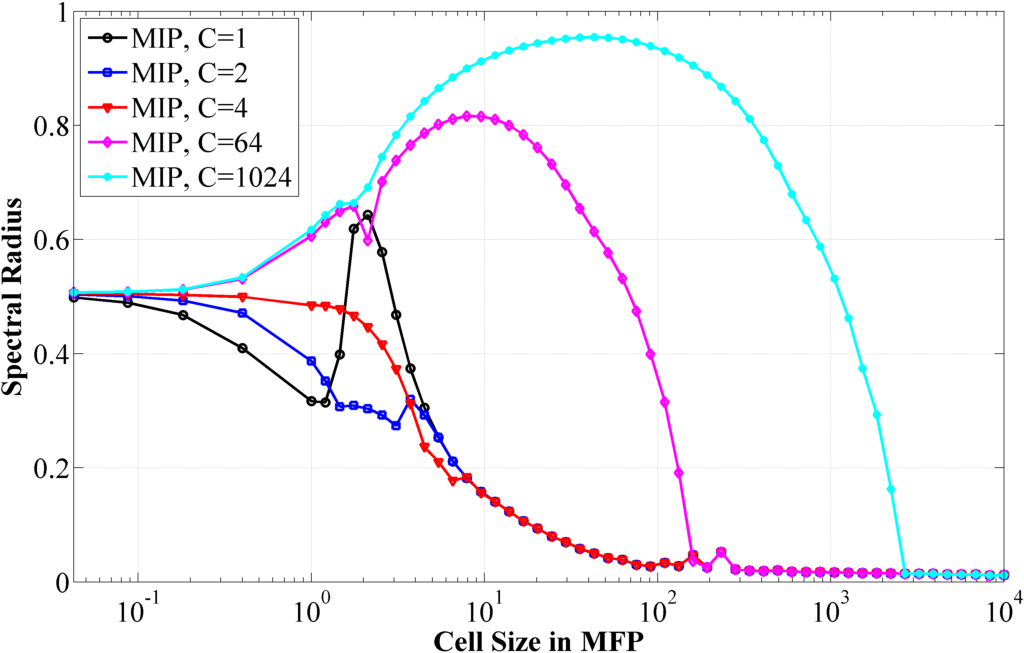
\includegraphics[width=0.9\textwidth]{figures/appendices/MIP_V_tri_LS8_C=1,2,4,64,1024.png}
\caption{Numerical spectral radius for the 2D MIP form using LS8 quadrature on triangles.}
\end{figure}

\begin{figure}
\label{fig::2D_NSR_MIP_polygons}
\centering
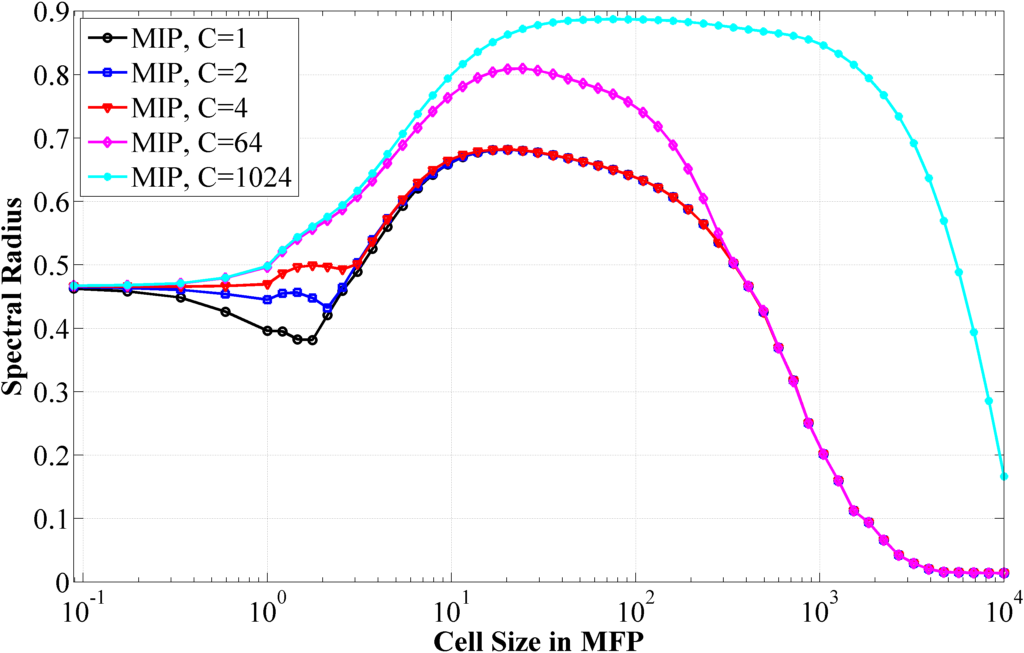
\includegraphics[width=0.9\textwidth]{figures/appendices/MIP_V_poly2D_LS8_C=1,2,4,64,1024.png}
\caption{Numerical spectral radius for the 2D MIP form using LS8 quadrature on polygons.}
\end{figure}

\begin{figure}
\label{fig::2D_NSR_MIP_q,t,p}
\centering
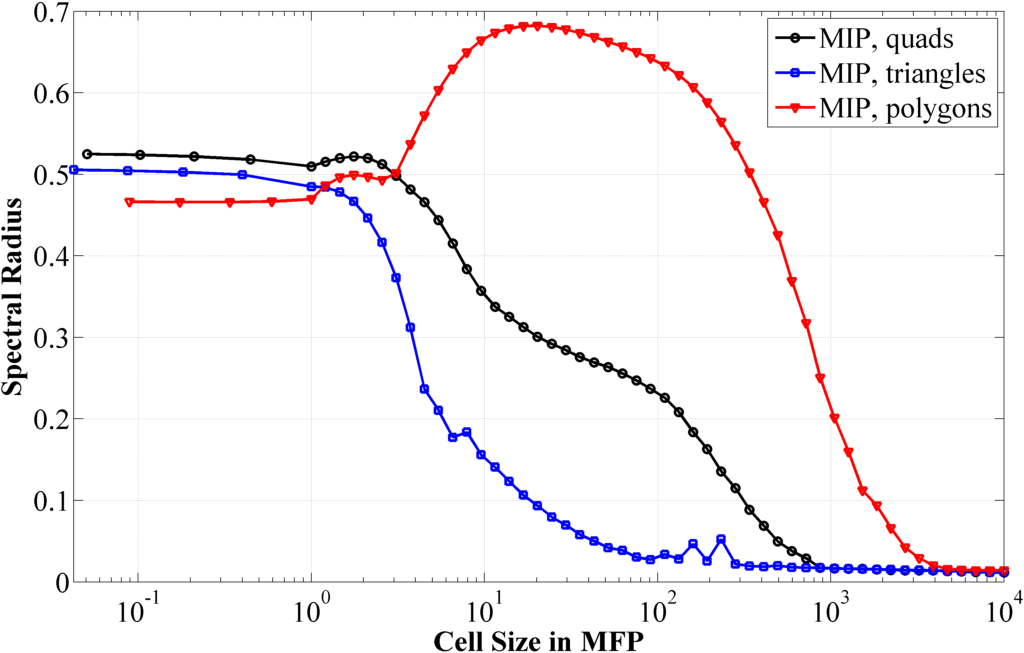
\includegraphics[width=0.9\textwidth]{figures/appendices/MIP_V_quad,tri,poly_LS8_C=4.png}
\caption{Numerical spectral radius for the 2D MIP form using LS8 quadrature on different mesh types with $C=4$.}
\end{figure}

% End: IP and MIP 2D NSR Plots
%%%%%%%%%%%%%%%%%%%%%%%%%%%%%%%%%%%%%%%%%%%%%%%%%%%%%%

